% English submission draft translated from the r21 Chinese master.
% See ../submission/source_binding.json for the exact source and figure hashes.
% Pending author declarations are deliberately marked AUTHOR INPUT REQUIRED.
\documentclass[preprint,12pt]{elsarticle}
\usepackage{fontspec}
\setmainfont{TeX Gyre Termes}
\usepackage{amsmath,amssymb}
\usepackage{booktabs,array,graphicx,float}
\usepackage{algorithm,algpseudocode}
\usepackage{hyperref,xurl}
\usepackage{microtype}
\usepackage{placeins}
\setlength{\emergencystretch}{2em}
\hypersetup{hidelinks,pdftitle={FAECO: Candidate Exploration and Failure Characterization for Pre-Placement Gate-Level Timing ECO},pdfauthor={Yalong Tong and Chang Liu}}
\biboptions{numbers,sort&compress}
\graphicspath{{../figures/manual/figures/}{../figures/data/final/}}
\newcommand{\AuthorInput}[1]{\textbf{AUTHOR INPUT REQUIRED:} #1}
\journal{Integration, the VLSI Journal}

\begin{document}
\begin{frontmatter}
\title{FAECO: Candidate Exploration and Failure Characterization for Pre-Placement Gate-Level Timing ECO\tnoteref{draftstatus}}
\tnotetext[draftstatus]{Submission draft. Author identities, correspondence, declarations, AI-use provenance and journal-specific requirements require author confirmation.}
\author[affiliation]{Yalong Tong\fnref{authorcheck}}
\author[affiliation]{Chang Liu}
\affiliation[affiliation]{organization={College of Computer Science, National University of Defense Technology},city={Changsha},postcode={410073},country={China}}
\fntext[authorcheck]{\AuthorInput{Confirm the English forms and order of the two names, identify the corresponding author, and confirm the contact address supplied in the Chinese master: chancews@qq.com.}}

\begin{abstract}
Timing closure has become a critical challenge in digital chip design as circuit scale and design complexity continue to grow. Engineering change order (ECO) techniques reduce the iteration cost of re-synthesis and physical implementation by applying localized modifications to an existing design. Among them, pre-placement gate-level timing ECO explores local netlist modifications before placement and routing, but its candidate space is limited and per-candidate evaluation is costly. FAECO is a framework for candidate exploration and failure characterization. It builds and ranks four types of local modification candidates---logic-equivalent replacement (R), gate sizing (G), buffer insertion (B), and joint modification (JOINT)---over the local logic around violating paths via a multi-feature weighted cut and a critical-path cover cut, characterizes candidate failures into six types used for search diagnosis and ablation analysis, and commits candidates round by round through function and structural checks, timing analysis and final equivalence checking. Its core idea is to organize the multi-type candidate space and the evaluation order so as to improve search efficiency under a limited verification budget. On ISCAS89, ITC-99 and PicoRV32, 8/8, 18/19 and 2/2 instances achieve pre-placement ideal-net WNS improvement (the third PicoRV32 module has no setup path and is excluded), with no regression on the rest. Under fixed weights and 20 rounds, mixed candidates improve WNS by 1.07\,ns on average versus 0.16\,ns for gate sizing alone. Ablations further analyze the effects of the failure-feedback mechanism and structure-resynthesis candidates on search performance. These results highlight the importance of candidate exploration and ranking in pre-placement ECO search.
\end{abstract}
\begin{keyword}
Gate-level timing ECO \sep Gate-level local modification \sep Multi-feature weighted cut \sep Typed failure characterization \sep Layered verification \sep Pre-placement timing optimization
\end{keyword}
\end{frontmatter}

\section{Introduction}
\subsection{Background and problem}
Timing closure is a major challenge in digital chip design as integrated circuits become larger and more complex. Engineering change order (ECO) techniques apply local modifications to an existing design, avoiding complete re-synthesis and physical implementation and reducing iteration cost. ECO can target either functional errors or timing violations. This work addresses gate-level timing ECO after synthesis and before placement and routing. A gate-level local modification applies an equivalent-cell replacement, gate sizing, buffer insertion, or a small combination of gate modifications within the fanin cone of violating logic in an already mapped netlist. Conventional timing ECO mainly uses buffer insertion (B) and gate sizing (G) to change driving capability and path load, improving worst negative slack (WNS) and total negative slack (TNS). For severe path violations, the capability of B/G optimization is limited, and structural remapping remains constrained by the available candidate space\cite{ho2010eco,liu2021rlsizer,chen2024aito}. The increasing cost of post-placement modifications makes early ECO exploration more valuable. However, physical information is unavailable before placement, and systematic choices of what to modify and in what order to evaluate the alternatives remain difficult.

Beyond B/G optimization, technology remapping and local logic patches expand the space of structural changes. These methods can change the local logic implementation but require additional functional-equivalence checks and candidate screening. The interaction between patch construction and physical optimization affects both verification cost and timing benefit.

Pre-placement gate-level timing ECO faces two related limitations: restricted candidate types and costly candidate evaluation. B/G modifications mainly change driving capability and load, while structural remapping needs an effective way to organize and rank many alternatives. Three questions follow: how to expand the local modification space for deep logic, how to control functional, timing and physical validation cost, and how to characterize candidate failures so that they inform search diagnosis. FAECO addresses candidate expansion through the exploration framework in Section~\ref{sec:mechanism}, evaluation cost through layered validation in Section~\ref{sec:validation}, and search analysis through typed failure characterization in Section~\ref{sec:failure_char}.

We define candidate exploration as the generation, screening and ranking of multiple types of local modification around violating logic windows. It organizes alternative structural changes and prioritizes candidates with timing potential under a limited validation budget. The central problem is therefore how to organize multiple local modification types and allocate finite validation resources effectively when physical information is incomplete.

\subsection{Motivation}
This work investigates how to construct additional local modification candidates within violating fanin cones and use critical-path information to arrange their evaluation order. Many candidates fail functional, structural or timing checks during the search. These failures characterize limitations of the current candidate space and ranking. FAECO uses a multi-feature weighted cut and a critical-path cover cut to generate candidates, and classifies validation failures to support subsequent search analysis.

The experiments use ISCAS89\cite{iscas89}, ITC-99\cite{itc99} and PicoRV32\footnote{\url{https://github.com/YosysHQ/picorv32}} netlists mapped to the public SKY130 HD standard-cell library. Ideal-net static timing analysis (STA) measures candidate timing benefit. Selected experiments also apply a simplified Standard Parasitic Exchange Format (SPEF) model, and independent sequential equivalence checking (SEC) evaluates the final repaired netlists.

\subsection{Contributions}
The work centers on candidate exploration for pre-placement gate-level timing ECO:
\begin{enumerate}
\item \textbf{A candidate exploration framework.} FAECO takes local windows around violating paths, constructs R/G/B/JOINT candidates using weighted and critical-path cover cuts, and combines cut cost, critical-path coverage and strategy priority to rank them. The design expands local modification alternatives and aims to reduce candidate evaluation cost in the absence of placement information.
\item \textbf{Failure characterization and search analysis.} Six failure classes cover local function/structure, boundary closure, candidate size, insufficient timing gain, validation timeout and parasitic re-evaluation. They identify search bottlenecks and provide evidence for refining candidate-generation strategies.
\end{enumerate}

A public-tool implementation and validation platform supports these contributions. Each accepted modification becomes the baseline for the next round, which extracts new violating cones and generates fresh candidates. Local function/structure checks, ideal-net STA and optional simplified SPEF re-evaluation precede final independent SEC. Across ISCAS89, ITC-99 and PicoRV32, 8/8, 18/19 and 2/2 assessable instances respectively obtain strict WNS improvement; the third PicoRV32 module has no setup path.

\section{Related work}
\subsection{Structural remapping and logic patches}
ECO research includes structural remapping, logic-patch construction, and B/G physical optimization. Structural remapping changes local cells and their implementation to improve timing. Some methods combine remapping with buffer insertion and sizing\cite{ho2010eco}, while symbolic sampling explores rectification points\cite{kravets2019symbolic}. FAECO uses Liberty function matching to screen replaceable cells before timing evaluation, and performs global SEC independently. Spare-cell allocation in\cite{ho2010eco} uses post-route load and spare-cell placement, whereas FAECO constructs candidates before placement. Symbolic sampling in\cite{kravets2019symbolic} expands the search space and uses validation results to screen rectification points.

Logic-patch methods typically extract a local window around a target rectification point, represent candidate logic with functionally reduced and-inverter graphs (FRAIGs), and use Boolean satisfiability (SAT) proofs to select functionally equivalent patches for functional repair\cite{jiang2010fraig,jiang2016resource}. Subsequent work incorporates resource cost into patch generation and uses SAT or combinational equivalence checking (CEC) for validation\cite{jiang2016resource,zhong2024stp}. FAECO brings computable local function-preservation information into candidate ranking and uses ideal-net timing as a separate acceptance signal. When equivalence validation fails, representative patch flows expand the window or patch size and enumerate again\cite{zhuo2018patch}, increasing construction and validation cost.

Recent B/G physical optimization includes gate sizing, joint B/G optimization and physically aware approaches\cite{liu2021rlsizer,huang2025phys,chen2024aito,zhang2025buffalo}. Learning-based methods further improve efficiency\cite{chen2024aito,zhang2025buffalo}. They primarily change driving capability and network load and generally do not reconstruct Boolean functions. FAECO constructs several local candidate types in violating fanin cones of mapped netlists and ranks them using critical-path information.

\subsection{B/G physical optimization and positioning}
Several related approaches use commercial EDA engines or internal industrial flows. We use public Yosys\footnote{\url{https://yosyshq.net/yosys/}}, OpenSTA\footnote{\url{https://github.com/parallaxsw/OpenSTA}} and OpenROAD\cite{openroad} tools to implement gate-level candidate search on SKY130 HD\footnote{\url{https://github.com/google/skywater-pdk}}. The flow covers mapped netlists, candidate construction, ideal-net STA, and post-placement/global-route parasitic estimation. Sequential experiments apply construction-level state-preservation checks, followed by independent whole-netlist SEC.

Structural remapping and B/G physical optimization are commonly used for physical adjustments after placement or during routing; logic-patch construction often performs functional repair between synthesis and placement. FAECO combines local modification of a mapped netlist with pre-placement timing screening, using ideal-net STA and a simplified wire-load model. Different input stages and evaluation goals impede direct quantitative comparisons, so the experiments use a common public mapping and constraint environment to investigate candidate spaces, evaluation order and cost. Tables~\ref{tab:related_diff} and~\ref{tab:baseline_cmp} summarize the methodological positioning and comparison constraints.

\begin{table}[htbp]
\centering\small
\caption{Main emphases of four method categories.}\label{tab:related_diff}
\begin{tabular}{p{0.20\linewidth}p{0.33\linewidth}p{0.37\linewidth}}\toprule
Method & Main characteristic & Target problem\\\midrule
Structural remapping & Changes local logic topology & Deep logic and structural timing violations\\
Logic patches & Local logic changes with SAT/CEC validation & Functional ECO or joint functional/timing repair\\
B/G optimization & Physical adjustments using drive/load information & Small post-placement timing violations\\
FAECO & Weighted-cut candidate generation and typed failure diagnosis & Local timing ECO on pre-placement mapped netlists\\\bottomrule
\end{tabular}
\end{table}

\begin{table}[htbp]
\centering\small
\caption{Main obstacles to direct quantitative comparisons.}\label{tab:baseline_cmp}
\begin{tabular}{p{0.25\linewidth}p{0.66\linewidth}}\toprule
Category & Comparison constraint\\\midrule
Structural remapping & Spare-cell allocation depends on post-route load and the spare-cell layout\\
Logic patches & Acceptance targets functional equivalence through SAT/CEC rather than WNS gain\\
B/G physical optimization & Learning-based methods require training environments/data; many physical flows use commercial engines or internal infrastructure\\
FAECO & Public tools and process library; scripts and parameters are intended for the supplementary package\\\bottomrule
\end{tabular}
\end{table}

\section{Method}
\subsection{Problem definition}
Given a mapped netlist $G'$, target period $T$, timing constraints and cell library $\mathcal L$, FAECO searches local candidates $p$ in fanin cones of violating endpoints to produce $G^*$. The main timing acceptance condition is $\Delta_{\mathrm{WNS}}(p)>0$. Independent SEC compares the final repaired netlist with the baseline. Optional physical gating adds the SPEF condition in Section~\ref{sec:validation}. Optional TNS-aware acceptance allows equal WNS with improved TNS.

The four transformations are R, a cross-equivalent-cell or logic-implementation replacement excluding pure drive-size changes; G, a drive-size change within the same functional cell family; B, an identity buffer insertion; and JOINT, joint enumeration. Sequential experiments do not modify flip-flops, clock or reset cells. A candidate comprises local gates and boundary ports and is generated only in combinational regions without tri-state, clock-gating or reset logic. Library function matching and structural rules screen constructions before final SEC. Table~\ref{tab:symbols} defines the main notation.

\begin{table}[htbp]
\centering\small
\caption{Notation.}\label{tab:symbols}
\begin{tabular}{p{0.30\linewidth}p{0.61\linewidth}}\toprule
Symbol & Definition\\\midrule
$G=(V,E)$ & Gate graph: gates/ports are vertices and signal connections are edges\\
$C(G,t)\subseteq V$ & Fanin cone of target output $t$\\
$K(G,t)$ & $s$--$t$ split graph with gate input/output capacity edges and fanin dependencies\\
$C_w$ & Weighted minimum-cut candidate boundary controlled by Eq.~\eqref{eq:cost}\\
$C_c$ & Critical-path cover boundary complementary to $C_w$; $\lambda_c$ affects cover ranking and depth discount\\
$\mathrm{cost}(v)$ & Node cost of gate $v$\\
$s(v),n_C,S_2$ & Local fanin-cone size; target-cone size $n_C=|C(G,t)|$; $S_2=\sum_u s(u)^2$\\
$\lambda_b,\lambda_s,\lambda_v,\lambda_c,\lambda_f$ & Search weights: boundary, size, verification and fanout terms enter node cost; $\lambda_c$ discounts depth in the denominator and adjusts cover ranking\\\bottomrule
\end{tabular}
\end{table}

\subsection{Overview}\label{sec:overview}
FAECO has three stages (Fig.~\ref{fig:method_flow}):
\begin{enumerate}
\item \textbf{Mapping preparation.} A two-step Yosys flow produces a SKY130 HD mapped netlist $G'$. Liberty provides cell functions and timing. Berkeley Logic Interchange Format (BLIF) normalization and ABC \texttt{cec}\cite{abc} support combinational checks.
\item \textbf{Cut-based candidate generation.} An $s$--$t$ split graph is built over $C(G,t)$. Liberty matching determines R availability; gates without R candidates receive less critical-path reward and fall back to G/B. Weighted and critical-path cover cuts generate candidates ranked by cut cost, coverage and strategy priority. OpenSTA supplies acceptance metrics. F1--F6 characterize failures and optionally update search weights.
\item \textbf{Validation and acceptance.} Function/structure screening precedes ideal-net WNS/TNS evaluation. With physical gating enabled, only ideal gains above 10\,ps enter simplified SPEF re-evaluation. Gains in $0<\Delta\mathrm{WNS}\le10$\,ps are filtered without F1--F6 feedback. F6 denotes a candidate satisfying the ideal acceptance predicate whose WNS does not improve under SPEF.
\end{enumerate}

\begin{figure}[htbp]\centering
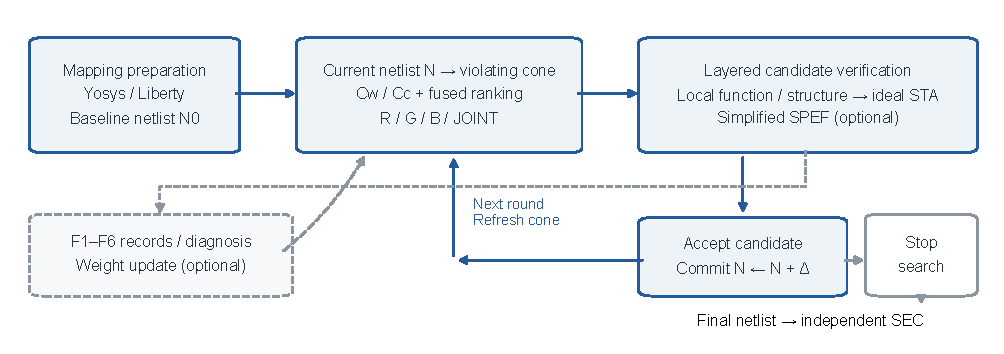
\includegraphics[width=\linewidth]{fig1_iterative_flow_r21.pdf}
\caption{Candidate evaluation and iterative submission. An accepted candidate becomes the next-round baseline, and the violating cone is extracted again. Dashed gray links denote failure recording and optional weight updates. Whole-netlist SEC is applied after search. This explanatory diagram was scripted with OpenAI Codex assistance; exact model/version: AUTHOR INPUT REQUIRED.}\label{fig:method_flow}
\end{figure}

\begin{algorithm}[htbp]\small
\caption{FAECO search and submission}\label{alg:main}
\begin{algorithmic}[1]
\Require Mapped netlist $G'$, timing constraints $T$, library $\mathcal L$
\Ensure Repaired netlist $G^*$, accepted candidate set $\mathcal A$
\State Save $G_0\gets G'$; initialize $N\gets G_0$, $G^*\gets G_0$, $\mathcal A\gets\emptyset$, weights $\lambda$
\Repeat
\State Extract the fanin cone of the worst violating endpoint in current $N$; partition by depth if needed
\State Generate and rank R/G/B/JOINT candidates using weighted and critical-path cover cuts
\State Perform local function/structure checks and OpenSTA measurements
\State Re-evaluate qualifying candidates under simplified SPEF when enabled
\State If a candidate satisfies Eq.~\eqref{eq:accept} and any enabled SPEF gate, add it to $\mathcal A$, submit $N\gets N+\Delta$, and update $G^*$. Candidates within a round share $N$ and do not accumulate. After submission, discard remaining candidates built from the previous $N$; regenerate them in the next round
\State Record F1--F6. If feedback is enabled, update subsequent search inputs/weights; fixed-weight runs only record failures. Candidates filtered by the 10\,ps threshold do not participate in feedback
\Until{Timing is met, candidates are exhausted, or a stopping condition holds}
\State \Return $G^*,\mathcal A$
\end{algorithmic}
\end{algorithm}

Algorithm~\ref{alg:main} describes search and submission; final SEC is separate. Multi-round repaired netlists accumulate accepted patches round by round, while the efficiency-first setting in Section~\ref{sec:eff_prio} runs once. Failure feedback updates weights after candidate evaluation and affects construction in the next round, without reordering candidates already generated for the current round. If a round exhausts candidates without acceptance and a stopping condition has not been reached, updated weights initiate another search round.

\subsection{Multi-type candidate exploration and ranking}\label{sec:mechanism}
\begin{figure}[htbp]\centering
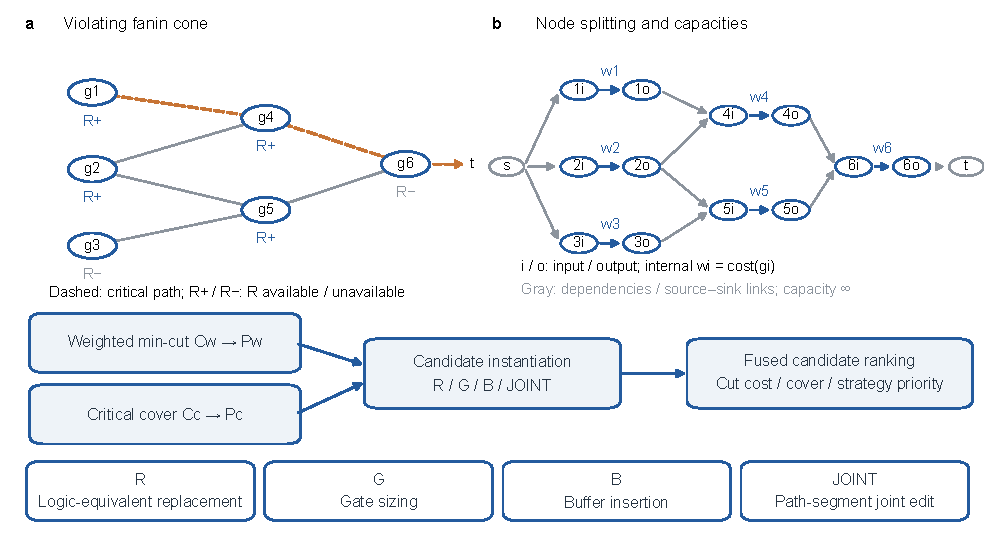
\includegraphics[width=\linewidth]{fig2_candidate_mechanism_r21.pdf}
\caption{Candidate construction and fused ranking. The six-gate cone and split graph have matching dependencies. Internal-edge capacities equal node costs; dependency and source/sink edges have infinite capacity. $C_w$ produces weighted boundaries, while $C_c$ supplements coverage candidates using cone criticality and R availability. The example illustrates construction relationships. This explanatory diagram was scripted with OpenAI Codex assistance; exact model/version: AUTHOR INPUT REQUIRED.}\label{fig:cut_generation}
\end{figure}

\subsubsection{Local window extraction}
As illustrated in Fig.~\ref{fig:cut_generation}, $C_w$ determines candidate boundaries, node cost guides selection/ranking within the boundary, and $C_c$ supplements critical-path coverage. Reverse traversal from a violating endpoint extracts a local combinational fanin cone $C(G,t)$. Gate annotations include R availability, critical-path coverage and candidate-size features.

\subsubsection{Candidate boundaries from complementary sources}
Weighted minimum-cut cost combines boundary, candidate-size, verification-cost and fanout features. For gates with R candidates, $\lambda_c$ introduces the depth discount in Eq.~\eqref{eq:cost}. The same weight adjusts ranking of complementary critical-path cover candidates. R availability controls candidate instantiation and strategy switching: when a gate has no R equivalent, its R-related coverage discount and fanout term are disabled and the search turns to G/B. The weighted boundary $C_w$ prioritizes local scale, while $C_c$ covers timing-critical gates.

\subsubsection{Fused candidate ranking}
Both boundary sets instantiate R/G/B/JOINT candidates. Fused ranking combines cut cost, coverage and strategy priority before OpenSTA measures WNS/TNS changes. The acceptance predicate retains effective candidates. Optional feedback updates the weights associated with F1--F6 for the next construction round; Section~\ref{sec:ablation} evaluates its search effect.

With identical SDC and clock constraints, candidate gain is
\begin{equation}\label{eq:dtiming}
\Delta_{\mathrm{WNS}}(p)=\mathrm{WNS}_{\mathrm{after}}(p)-\mathrm{WNS}_{\mathrm{before}}.
\end{equation}
Let $\mathrm{depth}(v)$ be cone logic depth, $V_R$ the gates with R candidates, and $\mathbb1[\cdot]$ the indicator. Node cost is
\begin{equation}\label{eq:cost}
\begin{aligned}
\mathrm{cost}(v)={}&\Big(1+\frac{\lambda_b}{1+\mathrm{depth}(v)}+\lambda_s\frac{s(v)^2}{S_2}
 +0.01\lambda_v n_C\\
 &+0.1\lambda_f\mathbb1[v\in V_R]\mathrm{fanout}(v)\Big)\\
 &\Big/\Big(1+\lambda_c\mathbb1[v\in V_R]\frac{\mathrm{depth}(v)}{\mathrm{depth}_{\max}}\Big).
\end{aligned}
\end{equation}
Boundary, size, verification and fanout weights are $\lambda_b,\lambda_s,\lambda_v,\lambda_f$; $\lambda_c$ controls the depth discount. All default to 1.0. Here $n_C=|C(G,t)|$, $s(v)$ is the local fanin-cone size of $v$, $S_2=\sum_u s(u)^2$, and $\mathrm{depth}_{\max}=\max_u\mathrm{depth}(u)$. The fanout term and depth discount apply only where R candidates exist. Other nodes remain available for G/B. $\lambda_c$ also adjusts critical-cover ranking toward highly critical nodes. Normalization controls preference for large cones. The fixed coefficients 0.01 and 0.1 scale verification-size and fanout terms and remain unchanged in all experiments.

\subsection{Feature motivation}\label{sec:feature_motivation}
Each cost feature addresses a common pre-placement ECO risk (Table~\ref{tab:feature_motivation}). Boundary features affect modification extent, size features discourage large local cones, verification features penalize cone size, fanout features lower priority of heavily loaded nodes, and depth features prioritize timing-critical logic. Fixed default weights are used without tuning by circuit or dataset.

\begin{table}[htbp]\centering\small
\caption{Weighted-cut features and ECO design considerations.}\label{tab:feature_motivation}
\begin{tabular}{p{0.15\linewidth}p{0.31\linewidth}p{0.44\linewidth}}\toprule
Feature & Cost term & Risk and design preference\\\midrule
Boundary & $\lambda_b/(1+\mathrm{depth})$ & Lower priority for candidates crossing local logic boundaries\\
Size & $\lambda_s s(v)^2/S_2$ & Prefer enumerable and assessable candidate scales\\
Verification & $0.01\lambda_v n_C$ & Penalize cone size as a verification-scale proxy\\
Fanout & $0.1\lambda_f\mathrm{fanout}$ & Lower priority for high-load nodes\\
Depth & $\lambda_c\mathrm{depth}/\mathrm{depth}_{\max}$ & Prioritize timing-critical coverage\\\bottomrule
\end{tabular}
\par\smallskip\footnotesize Fanout and depth terms are gated by R availability. The table summarizes the intended ranking roles of Eq.~\eqref{eq:cost}.
\end{table}

\subsection{Typed failure characterization and search analysis}\label{sec:failure_char}
Table~\ref{tab:failures} defines F1--F6 and their search-analysis actions. Fixed-weight runs only record failures. With feedback enabled, the corresponding weights increase by 1.0 per failure class; F5 also halves the maximum cone size. F6 records failure under simplified SPEF re-evaluation. An exponential moving average (EMA) variant smooths adaptive updates and is tested separately in Section~\ref{sec:ablation}.

\begin{table}[htbp]\centering\footnotesize
\caption{Failure classes and search-analysis actions.}\label{tab:failures}
\begin{tabular}{p{0.20\linewidth}p{0.32\linewidth}p{0.38\linewidth}}\toprule
Failure & Detection & Action when feedback is enabled\\\midrule
F1: local function/structure & Liberty function matching or structural checks fail & Increase $\lambda_b$ and $\lambda_f$, lowering high-fanout/boundary priority\\
F2: boundary & Cone boundary is not closed & Increase $\lambda_b$; tighten boundaries and retain mapped gates\\
F3: excessive size & Candidate exceeds the size threshold & Increase size penalty and prefer smaller cuts\\
F4: insufficient timing gain & Candidate fails Eq.~\eqref{eq:accept} & Increase $\lambda_c$ and critical-cover priority in the next round\\
F5: validation timeout & Local check or STA exceeds the per-candidate limit (default 60\,s) & Increase $\lambda_v$ and halve the maximum cone size\\
F6: wire-load timing failure & Physical gate enabled, ideal gain $>10$\,ps, but no SPEF WNS gain & Increase $\lambda_b$ and prefer smaller local boundaries\\\bottomrule
\end{tabular}
\end{table}

\subsection{Validation and acceptance}\label{sec:validation}
Local function and structure checks screen candidates before OpenSTA timing evaluation. R candidates use Liberty matching; G/B use function-preserving constructions. ABC \texttt{cec} can validate combinational netlists when enabled. The main and cross-dataset experiments apply independent SEC to each final baseline/repaired pair, separately from ideal-net candidate acceptance. Under SKY130 behavioral cell models, SEC checks combinational logic and state-transition relationships. OpenSTA measures ideal-net timing; the OpenROAD flow measures timing with global-route parasitic estimates.

Under the same SDC, clock and analysis corner,
\begin{equation}\label{eq:accept}
\begin{aligned}
\operatorname{Accept}(p)={}&[\Delta_{\mathrm{WNS}}(p)>0]\\
&\lor[\mathrm{tns\_aware}\land\Delta_{\mathrm{WNS}}(p)=0\\
&\qquad\land\Delta_{\mathrm{TNS}}(p)>0].
\end{aligned}
\end{equation}
With physical gating, candidates satisfying this predicate with ideal gain above 10\,ps enter SPEF re-evaluation. Gains in $(0,10]$\,ps are excluded from the final accepted set. Candidates with SPEF WNS improvement enter $\mathcal A$; otherwise F6 is recorded and optionally informs next-round search. Without the gate, SPEF is an independent re-evaluation and does not alter ideal-net acceptance.

\subsection{Construction complexity}\label{sec:impl}
The split graph uses max-flow/min-cut. For $n$ cone gates and $f$ dependency edges, there are $V=2n+2$ nodes and $E=O(n+f)$ edges. Edmonds--Karp costs $O(VE^2)$ per cut. This excludes candidate STA and final SEC, which dominate practical runtime; the individual cut solve contributes little. Reverse breadth-first search extracts $C(G,t)$. Large violating cones are partitioned by depth into sub-cones bounded by gate count, with independently generated candidates ranked along critical paths to control memory and solve size.

\subsection{AI-assisted research and figure preparation}
\AuthorInput{Confirm and complete the research-use record before submission.} OpenAI Codex assisted code implementation and inspection, test construction, experimental-workflow analysis, evidence-ledger audits, and reproducible Python figure scripts in the project records. These activities extend beyond language editing. Numerical plots are computed from archived EDA results; explanatory figures are drawn as editable vector diagrams. The tools did not serve as the timing or equivalence oracle: the reported measurements and proofs come from the EDA tools described above. Exact AI tools/models, versions, access dates, activities in earlier project stages, and the scope of human review must be supplied and confirmed by the authors. This draft does not assert that all generated code or interpretations have already been approved by both authors.

\section{Experiments}\label{sec:exp}
\subsection{Setup}\label{sec:setup}
\textbf{Environment and datasets.} Experiments ran in WSL2 (Ubuntu 24.04.4 LTS; kernel 6.6.87.2-microsoft-standard-WSL2) on an AMD Ryzen 7 7435H host, with 16 visible logical cores and 15\,GB memory. The main flow uses OSS-CAD Suite (Yosys 0.67+146, OpenSTA 3.1.0); SEC uses WSL Yosys 0.33. Datasets comprise eight ISCAS89 circuits, 19 ITC-99 circuits and three PicoRV32 modules, using a 0.5\,ns clock period to impose timing pressure. WNS improvement is the primary outcome under identical constraints. Other metrics are global-route-estimated WNS and candidate STA counts; TNS supports optional auxiliary acceptance. b06 retains equal-WNS/improved-TNS acceptance, which is excluded from strict-WNS improvement counts. TNS-aware acceptance is not combined with physical gating in these experiments.

\textbf{Inclusion.} ISCAS89 includes eight sequential circuits that map successfully through the common Yosys-to-SKY130 flow and have valid setup paths. ITC-99 includes b01--b15, b17 and b20--b22. b18 and b19 are separately reported large examples, outside the unified 19-circuit statistics. PicoRV32 includes its core, \texttt{picorv32\_pcpi\_mul} multiplier, and storage-dominated \texttt{picorv32\_regs}, covering control, arithmetic and storage structures.

\textbf{Configurations.} Section~\ref{sec:iscas} uses one round and stops after the first improvement; Section~\ref{sec:ood} permits eight rounds. Section~\ref{sec:ablation} compares strategy configurations under a 20-round limit and separately tests feedback. OpenROAD re-evaluates the accepted candidates from Section~\ref{sec:iscas}; SPEF scans/gating are separate experiments. Section~\ref{sec:s_boundary} evaluates local resynthesis. b17 has the timeout exception in Section~\ref{sec:itc99}. Table~\ref{tab:configs} summarizes settings. Scripts and parameters are intended for the supplementary package. Efficiency-first and unified cross-dataset results use archived runs whose code revision was not fully recorded; same-configuration reruns drift on some circuits. Feedback and S comparisons retain separate version/configuration records and must be reproduced using their own records.

\begin{table}[htbp]\centering\small
\caption{Efficiency-first and 20-round configurations.}\label{tab:configs}
\begin{tabular}{p{0.39\linewidth}p{0.22\linewidth}p{0.28\linewidth}}\toprule
Parameter & Efficiency-first & 20-round comparison\\\midrule
Maximum rounds & 1; stop after first gain & 20\\
F1--F6 feedback & Enabled & Disabled; fixed weights\\
10\,ps SPEF gate & Off & Off\\
Default per-candidate limit & 60\,s & 60\,s\\\bottomrule
\end{tabular}
\par\smallskip\footnotesize The strategy comparisons use a fixed-weight runner. Unified cross-dataset runs permit eight rounds and cross-round feedback. In the one-round setting, any weight update cannot affect subsequent candidate construction. b17's 180\,s exception belongs to the cross-dataset study.
\end{table}

Except for b06's auxiliary TNS acceptance, the primary criterion is strict WNS improvement in Eq.~\eqref{eq:accept}. Table~\ref{tab:overview} reports unified outcomes.
\begin{table}[htbp]\centering\small
\caption{Unified cross-dataset outcomes.}\label{tab:overview}
\begin{tabular}{lrrrr}\toprule
Dataset & Instances & Strict gain & Mean/median gain (ns) & SEC proven\\\midrule
ISCAS89 & 8 & 8/8 & 0.16/0.10 & 8/8\\
ITC-99 & 19 & 18/19 & 0.43/0.18 & 18/19\\
PicoRV32 & 3 & 2/2 & 0.60/0.60 & 2/2\\\bottomrule
\end{tabular}
\par\smallskip\footnotesize Up to eight rounds with cross-round feedback; gains refer to pre-placement ideal nets. Statistics use assessable instances. SEC counts completely proven modified pairs; b17 has one unproven point. The register-bank module has no register-to-register setup path and is excluded from gain and SEC denominators.
\end{table}

\subsection{Single-round repair quality and efficiency}\label{sec:iscas}
The single-round study evaluates repair quality and efficiency. Figure~\ref{fig:iscas_main} compares baseline and repaired ISCAS89 netlists; all eight improve strictly under ideal-net OpenSTA. R/G/B/JOINT constructions preserve flip-flops, clock and reset logic. All final pairs pass independent SEC (Table~\ref{tab:sec_iscas8}). Accepted candidate types are JOINT for s27/s382/s420/s953, G for s641/s713/s832, and R for s820; no standalone B candidate is accepted. This is the efficiency-first configuration\label{sec:eff_prio}, with the 10\,ps physical gate disabled. Thus s420's +0.01\,ns candidate is accepted under $\Delta\mathrm{WNS}>0$. The stopping condition differs from the subsequent multi-round study, so results are reported separately. JOINT combines local implementation and drive changes; G changes drive strength; R depends on equivalent Boolean implementations available in the library.

\begin{figure}[htbp]\centering
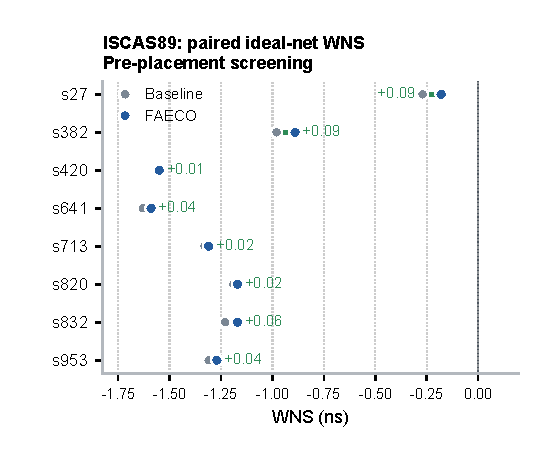
\includegraphics[width=0.78\linewidth]{fig3_single_round_r21.pdf}
\caption{Baseline and FAECO WNS on ISCAS89 sequential circuits at 0.5\,ns. Labels report gain relative to baseline.}\label{fig:iscas_main}
\end{figure}
\begin{table}[htbp]\centering\small
\caption{Gate-level sequential equivalence checks on ISCAS89.}\label{tab:sec_iscas8}
\begin{tabular}{lrrr}\toprule
Circuit & Equivalence cells & SEC & Time (s)\\\midrule
s27 & 11 & Proven & 0.303\\
s382 & 90 & Proven & 0.382\\
s420 & 79 & Proven & 0.368\\
s641 & 124 & Proven & 0.381\\
s713 & 126 & Proven & 0.410\\
s820 & 138 & Proven & 0.454\\
s832 & 145 & Proven & 0.437\\
s953 & 228 & Proven & 0.537\\\bottomrule
\end{tabular}
\par\smallskip\footnotesize Yosys \texttt{equiv\_make}, \texttt{equiv\_simple} and \texttt{equiv\_induct}; all eight pass under SKY130 behavioral cell models.
\end{table}

\subsection{Cross-dataset evaluation}\label{sec:ood}
\subsubsection{ITC-99}\label{sec:itc99}
Eighteen of the 19 unified ITC-99 circuits obtain strict WNS gain, while b06 remains unchanged; none regresses. At the default 60\,s per-candidate limit, b17 candidates time out as F5. Increasing only b17's limit to 180\,s yields +0.38\,ns within 104 candidate evaluation records, accepting a G replacement from \texttt{nor4b\_1} to \texttt{nor4b\_2}. The larger included circuits b14/b15/b17/b20/b21/b22 all improve. b06 has baseline WNS=-0.56\,ns and several adjacent \texttt{or4b\_1} gates on its critical path. In this R/G/B/JOINT search, G replacements are constrained by input-capacitance changes, and B/R do not yield an effective gain. No strict WNS improvement is observed in 664 candidate evaluation records.

G dominates accepted modifications: 17 circuits contain G acceptances (69 in total), while B and R occur in 14 and ten circuits. b20 and b21 have the largest gains, +1.98 and +2.75\,ns, mainly from G with additional R modifications. The 19-circuit set contains 3363 candidate evaluation records, of which 2994 STA results can be independently traced to unique candidate reports (2890 in the 18-circuit archive and 104 recovered for b17). This is an identifiable result count; the historical archives do not record all timeout launches, baseline analyses or cone refreshes. Median and mean gain are +0.18 and +0.43\,ns; b20/b21, whose baseline WNS is at most -13\,ns, account for much of the difference. Table~\ref{tab:f16_dist} reports failure triggers and provides search-diagnostic evidence.

Two separate large examples are outside these 19-circuit statistics. Mapped b18 has 75,700 cells approximately, with WNS changing from -13.34 to -13.27\,ns at 0.5\,ns in 24 candidate-level STA measurements. b19 has approximately 151,000 cells, changing from -17.44 to -16.00\,ns in 59 measurements.

\subsubsection{PicoRV32 modules}
Three structurally different modules from one RTL source reuse the ISCAS89 flow. The core and \texttt{picorv32\_pcpi\_mul} have valid setup paths and improve by +1.13 and +0.07\,ns through accumulated R/G/B modifications. The storage-bank module has no assessable setup path and is not repaired or included in improvement counts.

Unified strict-WNS improvement fractions are 8/8, 18/19 and 2/2. SEC considers 30 instances: 29 have actual netlist modifications, and 28/29 modified pairs are completely proven. b06's buffer/delay patches leave WNS unchanged and pass SEC. The unmodified register bank remains identical to baseline. b17 proves 12,812 equivalence points with \texttt{equiv\_simple} and \texttt{equiv\_induct}, leaving one point unproven; it corresponds to the same-function \texttt{nor4b\_1} to \texttt{nor4b\_2} sizing change and is reported separately. Figure~\ref{fig:unified_gain} shows all assessable instances.

\begin{figure}[htbp]\centering
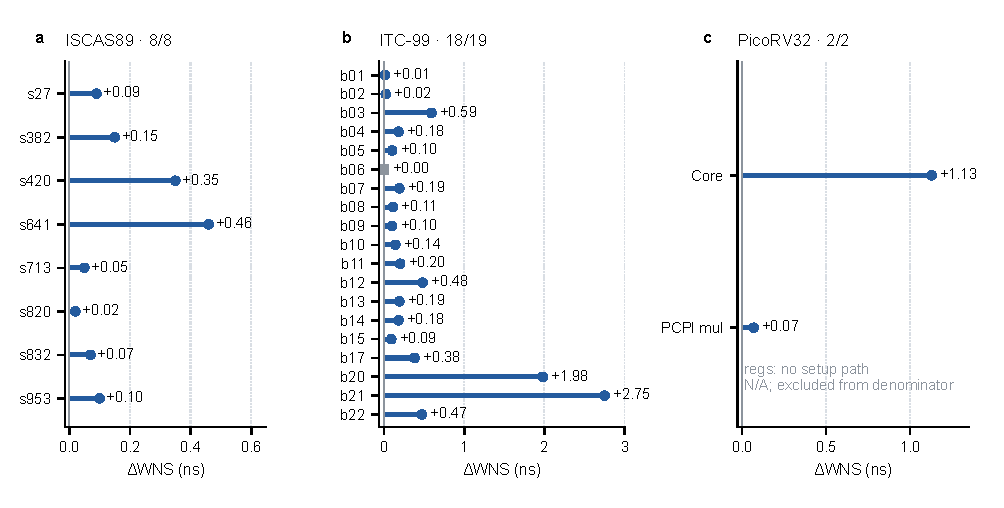
\includegraphics[width=\linewidth]{fig4_unified_gain_r21.pdf}
\caption{Per-instance ideal-net WNS gain under the unified iterative setting. Panel ranges differ. b17 uses a 180\,s candidate limit; the default is 60\,s. The register bank is excluded because it has no setup path. Results describe single archived runs.}\label{fig:unified_gain}
\end{figure}

\subsection{Candidate-space, ranking and feedback comparisons}\label{sec:ablation}
The first experiment uses an archived critical-instance strategy-enumeration runner under a 20-pass limit (Table~\ref{tab:ablation}), with first-improvement cost in Table~\ref{tab:efficiency}. It enumerates candidates and submits changes instance by instance within a pass, without the weighted or cover cuts in Eq.~\eqref{eq:cost}. The mixed configuration uses auxiliary TNS acceptance and R/G/B/JOINT; the randomized configuration enumerates R/G/B only. Their differences therefore reflect the joint effects of candidate construction and evaluation order.

With fixed search weights, mixed strategies average 1.07\,ns gain versus 0.16\,ns for G alone, 0.54\,ns for B alone and 0.40\,ns for the three randomized seeds. The shared 20-pass limit does not imply equal actual STA consumption. In six of seven circuits with ledgers, the mixed strategy reaches its first gain before the random-seed mean; s713 is the exception. First-improvement cost varies by up to sevenfold between seeds. The comparison describes strategy-level outcomes and startup cost; separate controls in the same runner are still needed to isolate weighted and cover cuts.

The second experiment isolates EMA feedback, holding candidate space, initial weights and the runner's STA reservation cap of 500 fixed. Fixed and Adaptive permit 20 rounds with early stopping. Let $B(k)$ be the best WNS gain through the $k$th new STA measurement. Final gain, first-improvement position and maximum $B(k)$ agree for the two configurations on all eight circuits; EMA provides no additional observed benefit. F1--F6 are therefore used for failure classification and search analysis. Table~\ref{tab:runtime} gives the cost to reach these endpoints and includes randomized ordering.

Figure~\ref{fig:budget_curves} plots this second experiment against new STA measurements. Fixed and EMA accumulate similar gains but stop at different positions. Randomized outcomes differ by circuit and seed; all three s953 randomized endpoints exceed Fixed. Natural endpoints distinguish terminal quality from measurement cost.

\begin{figure}[htbp]\centering
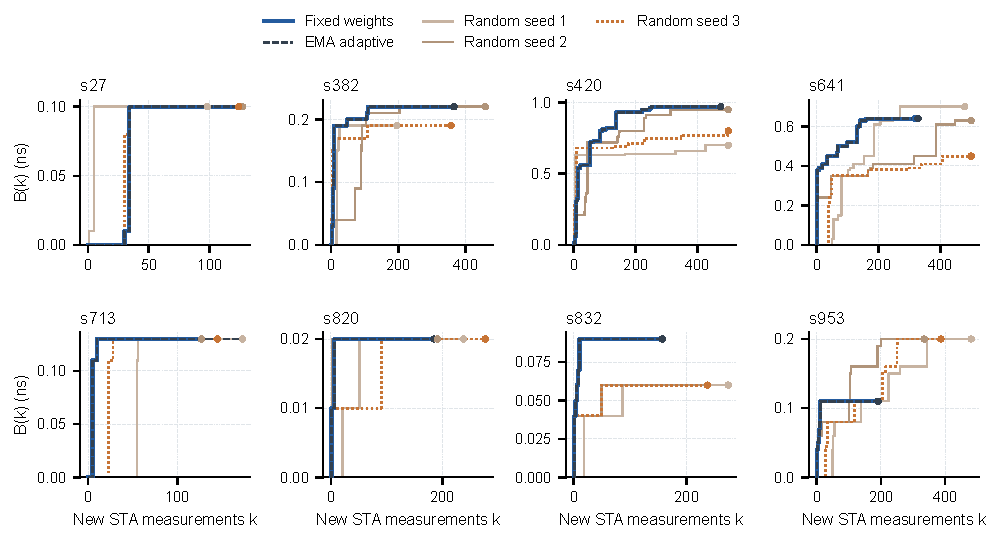
\includegraphics[width=\linewidth]{fig5_budget_curves_r21.pdf}
\caption{Gain accumulation in the same-runner feedback comparison. $k$ counts new STA measurements reconstructed from records with STA provenance and no cache-replay marker; pre-STA rejections and cache hits are excluded. Dots mark natural endpoints; curves do not extrapolate. All eight circuits and three random seeds are shown without cross-circuit averaging or interpolation. The per-circuit reservation cap is 500; baseline STA and final SEC are excluded. This family is separate from Table~\ref{tab:ablation}.}\label{fig:budget_curves}
\end{figure}

\begin{table}[htbp]\centering\small
\caption{WNS gains of local modification strategies on ISCAS89 (0.5\,ns).}\label{tab:ablation}
\begin{tabular}{lrrrr}\toprule
Circuit & G only & B only & Random & Mixed, 20 passes\\\midrule
s27 & +0.09 & +0.28 & +0.28 & +0.28\\
s382 & +0.17 & +0.19 & +0.19 & +1.00\\
s420 & +0.35 & +1.00 & +1.15 & +1.54\\
s641 & +0.45 & +1.27 & +0.57 & +1.63\\
s713 & +0.05 & +0.99 & +0.64 & +1.33\\
s820 & +0.02 & +0.26 & +0.15 & +0.99\\
s832 & +0.07 & +0.06 & +0.08 & +0.57\\
s953 & +0.09 & +0.24 & +0.12 & +1.25\\\midrule
Mean & 0.16 & 0.54 & 0.40 & 1.07\\\bottomrule
\end{tabular}
\par\smallskip\footnotesize Gains are in ns. Random contains R/G/B, shuffles candidates within each instance, and averages seeds 1/2/3. Mixed additionally contains JOINT. None updates F1--F6 weights; all have the same pass limit but different STA consumption. Mixed retains equal-WNS/improved-TNS acceptance. Complete invocation commands were not archived for every arm.
\end{table}

\begin{table}[htbp]\centering\small
\caption{Candidate-level STA count to the first improvement (0.5\,ns).}\label{tab:efficiency}
\begin{tabular}{lrrrrr}\toprule
Circuit & Mixed & Seed 1 & Seed 2 & Seed 3 & Random mean\\\midrule
s27 & 1 & 3 & 3 & 1 & 2.3\\
s382 & --- & 6 & 3 & 8 & 5.7\\
s420 & 2 & 5 & 1 & 1 & 2.3\\
s641 & 1 & 7 & 5 & 1 & 4.3\\
s713 & 7 & 1 & 5 & 2 & 2.7\\
s820 & 1 & 1 & 3 & 1 & 1.7\\
s832 & 1 & 1 & 2 & 1 & 1.3\\
s953 & 1 & 3 & 1 & 1 & 1.7\\\bottomrule
\end{tabular}
\par\smallskip\footnotesize Entries are cumulative candidate ordinals at the first result strictly above baseline. Mixed is lower than the random mean in six of seven assessable ledgers; s713 is the exception. Seeds vary by up to sevenfold. The mixed s382 ledger is missing. This archived 20-pass enumeration study has different candidate types between Mixed and Random.
\end{table}

\begin{table}[htbp]\centering\small
\caption{Candidate accounting and search time for the 20-round feedback study.}\label{tab:runtime}
\begin{tabular}{lrrr}\toprule
Configuration & New STA & Evaluation records & Time (s)\\\midrule
Fixed weights & 1947 & 4146 & 2010.8\\
EMA adaptive & 2003 & 4883 & 2065.3\\
Random, three-seed mean & 2480.7 & 5624 & 2460.3\\\bottomrule
\end{tabular}
\par\smallskip\footnotesize All arms permit 20 rounds with early stopping and 500 STA reservations per circuit. New STA excludes provenance-bearing cache replay; evaluation records also include pre-STA rejection. Fixed/EMA totals sum eight circuits. Random averages totals 2439/2476/2527 across seeds. Time includes construction, mapping and candidate STA, excluding final SEC. This configuration differs from Tables~\ref{tab:ablation} and~\ref{tab:efficiency}.
\end{table}

\begin{table}[htbp]\centering\small
\caption{Failure triggers in the ITC-99 main study.}\label{tab:f16_dist}
\begin{tabular}{lrrrrrr}\toprule
 & F1 & F2 & F3 & F4 & F5 & F6\\\midrule
Triggers & 138 & 3 & 16 & 2434 & 915 & 0\\\bottomrule
\end{tabular}
\par\smallskip\footnotesize Nineteen circuits and 4044 candidate evaluations. F4 accounts for 60.2\%; F6 is zero because the physical gate is disabled. This distribution retains b17's default 60\,s batch with 785 evaluations. Unified outcomes and 3363 evaluation records instead use its 180\,s rerun with 104 evaluations.
\end{table}

\subsection{Physical relevance of pre-placement screening}\label{sec:phys_closure}
This study examines whether the efficiency-first candidate gains persist after placement/global-route parasitic estimation (Fig.~\ref{fig:physical_transfer}). These candidates are separate from the 20-round study. Table~\ref{tab:pr8} shows that five of eight ISCAS89 circuits improve, one is unchanged, and two regress by 0.02 and 0.01\,ns. The flow uses OpenROAD 2.0, SKY130 HD and a 0.5\,ns clock. SPEF load scans/gating separately characterize wire-load sensitivity and F6. The OpenROAD results are post-hoc timing estimates used to assess stability under estimated parasitics.

\begin{figure}[htbp]\centering
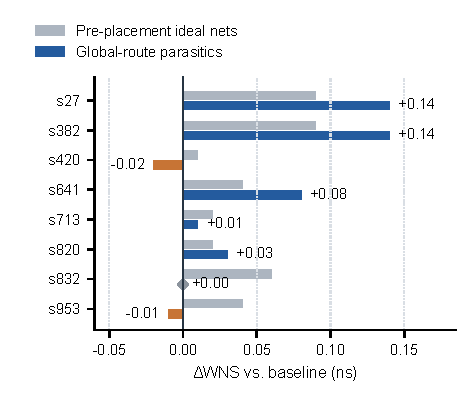
\includegraphics[width=0.72\linewidth]{fig6_physical_transfer_r21.pdf}
\caption{Gain retention for efficiency-first candidates. Each pair uses the same circuit/candidate, referenced to its baseline under ideal-net and global-route-estimated parasitics. All eight circuits are included: five improve, one is unchanged, and two regress; orange denotes regression and the diamond denotes no change. This one-round family is separate from Fig.~\ref{fig:unified_gain}.}\label{fig:physical_transfer}
\end{figure}

Independent SPEF scans show that ideal gains of an s382 R candidate and a b18 JOINT candidate approach zero as estimated wire length increases. At 40\,$\mu$m/unit, where a unit accumulates relative topological/Manhattan length after fanout, each net $e$ uses
\begin{equation}
L_{\mathrm{est}}(e)=40\,\mu\mathrm{m}\cdot u(e),\qquad R_e=r_{\mathrm{unit}}L_{\mathrm{est}},\quad C_e=c_{\mathrm{unit}}L_{\mathrm{est}}.
\end{equation}
Representative SKY130 HD \texttt{li1} RC values define the simplified SPEF. Fifty s382 candidates and six b18 candidates fail re-evaluation and are recorded as F6. Under enabled feedback, those failures inform subsequent search analysis. The gate identifies candidates whose WNS gains vanish under this load estimate.

\begin{table}[htbp]\centering\small
\caption{WNS after placement/global-route parasitic estimation.}\label{tab:pr8}
\begin{tabular}{lrrrrr}\toprule
 & \multicolumn{2}{c}{Pre-placement} & \multicolumn{2}{c}{Global-route estimate} & \\
\cmidrule(lr){2-3}\cmidrule(lr){4-5}
Circuit & Baseline & Repair & Baseline & Repair & Gain\\\midrule
s27 & -0.27 & -0.18 & -0.36 & -0.22 & +0.14\\
s382 & -0.98 & -0.89 & -1.16 & -1.02 & +0.14\\
s420 & -1.56 & -1.55 & -1.80 & -1.82 & -0.02\\
s641 & -1.63 & -1.59 & -2.10 & -2.02 & +0.08\\
s713 & -1.33 & -1.31 & -1.59 & -1.58 & +0.01\\
s820 & -1.19 & -1.17 & -1.52 & -1.49 & +0.03\\
s832 & -1.23 & -1.17 & -1.51 & -1.51 & 0.00\\
s953 & -1.31 & -1.27 & -1.60 & -1.61 & -0.01\\\bottomrule
\end{tabular}
\par\smallskip\footnotesize All values are ns; mapped inputs and accepted candidates match the pre-placement study. s27 uses 10\% floorplan utilization. Gain is repaired-minus-baseline WNS under global-route parasitic estimation.
\end{table}

\subsection{Structural candidate expansion and capability boundary}\label{sec:s_boundary}
In addition to R/G/B/JOINT constructions, a window-local structural resynthesis candidate S tests whether further structural change adds WNS benefit. Enlarging the S pool and disabling S provide controls. Disabling S reproduces the original endpoint on all eight circuits; non-S candidate sequences agree between arms and the STA cap is not reached. Table~\ref{tab:s_boundary} and Fig.~\ref{fig:s_candidate_outcomes} distinguish depth changes from timing outcomes.

\begin{figure}[htbp]\centering
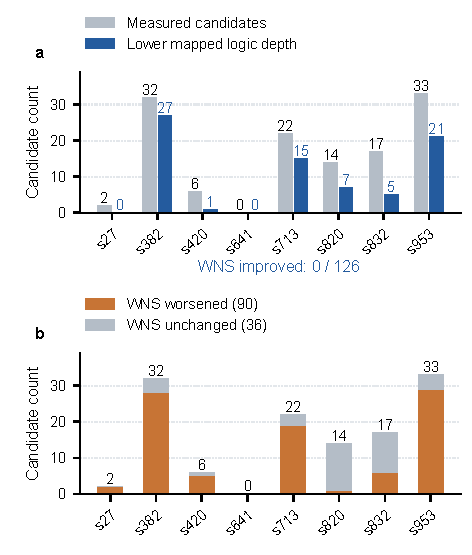
\includegraphics[width=0.70\linewidth]{fig7_s_boundary_r21.pdf}
\caption{Expanded S-candidate outcomes. The top panel compares measured candidates with those reducing mapped logic depth; the bottom divides WNS-unchanged and WNS-worsened candidates. These are separate classifications of the same 126 candidates. All eight circuits are shown; s641 has no successfully extracted window. Seventy-six candidates reduce depth, none improves WNS, and the paired S on/off endpoints agree on all eight circuits.}\label{fig:s_candidate_outcomes}
\end{figure}

\begin{table}[htbp]\centering\small
\caption{Capability boundary of structural candidates.}\label{tab:s_boundary}
\begin{tabular}{lrr}\toprule
Metric & Original pool & Expanded pool\\\midrule
S candidates & 37 & 126\\
$\Delta L>0$ & --- & 76/126\\
$\Delta_{\mathrm{WNS}}>0$ & 0 & 0/126\\
$\Delta_{\mathrm{WNS}}=0$ & --- & 36/126\\
$\Delta_{\mathrm{WNS}}<0$ & --- & 90/126\\
Circuits accepting S & 0/8 & 0/8\\\bottomrule
\end{tabular}
\par\smallskip\footnotesize $\Delta L=L_{\mathrm{before}}-L_{\mathrm{after}}$ is mapped-depth reduction; $\Delta_{\mathrm{WNS}}=\mathrm{WNS}_{\mathrm{after}}-\mathrm{WNS}_{\mathrm{before}}$. Depth and timing classifications are separate and can overlap, so all rows are not additive.
\end{table}

Expanding the pool increases S candidates from 37 to 126. Seventy-six reduce mapped depth, but none obtains strict WNS gain; 90 worsen WNS and 36 leave it unchanged. Under this window construction, resynthesis and mapping flow, pool expansion adds no WNS benefit. S remains optional and is excluded from the main performance contribution.

\FloatBarrier
\section{Conclusion}\label{sec:conclusion}
FAECO constructs R/G/B/JOINT candidates through weighted and critical-path cover cuts, combining failure characterization, iterative submission and layered validation for local pre-placement timing optimization. In the fixed-weight strategy study, mixed candidates average 1.07\,ns WNS gain versus 0.16\,ns for G alone. Cross-dataset evaluation demonstrates gains across multiple circuit families. In archived strategy comparisons, mixed candidates reach first improvement earlier than randomized strategies on most circuits, reflecting the joint effects of candidate construction and evaluation order.

EMA does not add observed benefit over fixed weights, and expanded S candidates do not improve WNS despite reducing some mapped depths. After OpenROAD placement/global-route estimation, five circuits retain gains, one is unchanged and two regress by at most 0.02\,ns. Insufficient timing gain dominates recorded failures (F4: 60.2\% of evaluations), providing direction for candidate-space design. Within these experiments, organizing the candidate space and evaluation strategy offers a route to better pre-placement ECO outcomes beyond reliance on a single modification type. The public-tool implementation provides a basis for reproducible study of automated ECO search.

\section*{Author contributions}
\AuthorInput{Supply and approve CRediT roles for Yalong Tong and Chang Liu. This draft does not assign roles or attest joint approval.}

\section*{Funding}
\AuthorInput{Provide funder names, grant numbers and funder roles, or confirm that no specific funding was received.}

\section*{Declaration of competing interest}
\AuthorInput{Each author must confirm relevant financial/non-financial interests. A no-conflict statement has not been assumed.}

\section*{Data availability}
The study uses public ISCAS89, ITC-99, PicoRV32 and SKY130 inputs, with project-specific mapped netlists, candidate records and analysis scripts. \AuthorInput{Provide the public archival repository, persistent identifier, release/commit, licenses and access conditions for the reproducibility package. The package has not been represented here as already publicly deposited.}

\section*{Ethics declaration}
\AuthorInput{Confirm whether institutional ethics approval is applicable and provide the appropriate statement. The described experiments concern public digital-circuit benchmarks and EDA outputs; no human-subject approval statement is inferred.}

\section*{Declaration of generative AI and AI-assisted technologies in the manuscript preparation process}
OpenAI Codex assisted English translation, manuscript organization, consistency checking, LaTeX preparation and reproducible figure-label adaptation. AI assistance also extended to research software and evidence analysis, as identified in the Methods record. \AuthorInput{Confirm every tool/model/version used, any other manuscript or research activities, and the extent of human review. Replace this draft only after the authors have reviewed the scientific content, verified the outputs and approved their accountability statement.}

% Retained bibliography entries and keys from the Chinese master.
\begin{thebibliography}{99}
\bibitem{ho2010eco} Ho K H, Chen Y P, Fang J W, et al. ECO timing optimization using spare cells and technology remapping[J]. IEEE Transactions on Computer-Aided Design of Integrated Circuits and Systems, 2010, 29(5): 697-710. DOI: 10.1109/TCAD.2010.2043573.
\bibitem{liu2021rlsizer} Lu Y C, Nath S, Khandelwal V, et al. RL-Sizer: VLSI gate sizing for timing optimization using deep reinforcement learning[C] //Proceedings of the 58th ACM/IEEE Design Automation Conference. Piscataway: IEEE, 2021: 733-738. DOI: 10.1109/DAC18074.2021.9586138.
\bibitem{chen2024aito} Wu H, Huang Z, Li X, et al. AiTO: Simultaneous gate sizing and buffer insertion for timing optimization with GNNs and RL[J]. Integration, the VLSI Journal, 2024, 98: 102211. DOI: 10.1016/j.vlsi.2024.102211.
\bibitem{iscas89} Brglez F, Bryan D, Kozminski K. Combinational profiles of sequential benchmark circuits[C] //Proceedings of IEEE International Symposium on Circuits and Systems. Piscataway: IEEE, 1989: 1929-1934. DOI: 10.1109/ISCAS.1989.100747.
\bibitem{itc99} Davidson S. ITC'99 benchmark circuits - preliminary results[C] //Proceedings of IEEE International Test Conference. Piscataway: IEEE, 1999: 1125. DOI: 10.1109/TEST.1999.805857.
\bibitem{kravets2019symbolic} Kravets V N, Lee N Z, Jiang J H R. Comprehensive search for ECO rectification using symbolic sampling[C] //Proceedings of the 56th Annual Design Automation Conference. New York: ACM, 2019: 71:1-71:6. DOI: 10.1145/3316781.3317790.
\bibitem{jiang2010fraig} Wu B H, Yang C J, Huang C Y, et al. A robust functional ECO engine by SAT proof minimization and interpolation techniques[C] //Proceedings of IEEE/ACM International Conference on Computer-Aided Design. Piscataway: IEEE, 2010: 729-734. DOI: 10.5555/2133429.2133584.
\bibitem{jiang2016resource} Cheng A C, Jiang I H R, Jou J Y. Resource-aware functional ECO patch generation[C] //Proceedings of the Design, Automation \& Test in Europe Conference \& Exhibition. Piscataway: IEEE, 2016: 1036-1041. DOI: 10.5555/2971808.2972050.
\bibitem{zhong2024stp} Pan H, Zhang R, Xia Y, et al. A semi-tensor product based circuit simulation for SAT-sweeping[C] //Proceedings of the Design, Automation \& Test in Europe Conference \& Exhibition. Piscataway: IEEE, 2024: 1-6. DOI: 10.23919/DATE58400.2024.10546678.
\bibitem{zhuo2018patch} Dao A Q, Lee N Z, Chen L C, et al. Efficient computation of ECO patch functions[C] //Proceedings of the 55th Annual Design Automation Conference. New York: ACM, 2018: 1-6. DOI: 10.1145/3195970.3196039.
\bibitem{huang2025phys} Ye Y, Xu P, Ren L, et al. Learning-driven physically aware large-scale circuit gate sizing[J]. IEEE Transactions on Computer-Aided Design of Integrated Circuits and Systems, 2025, 44(5): 1901-1914. DOI: 10.1109/TCAD.2024.3488577.
\bibitem{zhang2025buffalo} Hsiao H H, Lu Y C, Lim S K, et al. BUFFALO: PPA-configurable, LLM-based buffer tree generation via group relative policy optimization[C] //Proceedings of IEEE/ACM International Conference on Computer-Aided Design. Piscataway: IEEE, 2025: 1-9. DOI: 10.1109/ICCAD66269.2025.11240744.
\bibitem{openroad} Ajayi T, Chhabria V A, Fogaça M, et al. Toward an open-source digital flow: First learnings from the OpenROAD project[C] //Proceedings of the 56th ACM/IEEE Design Automation Conference. New York: ACM, 2019: 1-4. DOI: 10.1145/3316781.3326334.
\bibitem{abc} Brayton R, Mishchenko A. ABC: An academic industrial-strength verification tool[C] //Proceedings of the 22nd International Conference on Computer Aided Verification. Berlin: Springer, 2010: 24-40. DOI: 10.1007/978-3-642-14295-6\_5.
\end{thebibliography}

\end{document}
